\documentclass[tikz,border=10pt]{standalone}
\usepackage{times}
\usepackage{tikz}
\usetikzlibrary{positioning,arrows.meta,calc}
\begin{document}
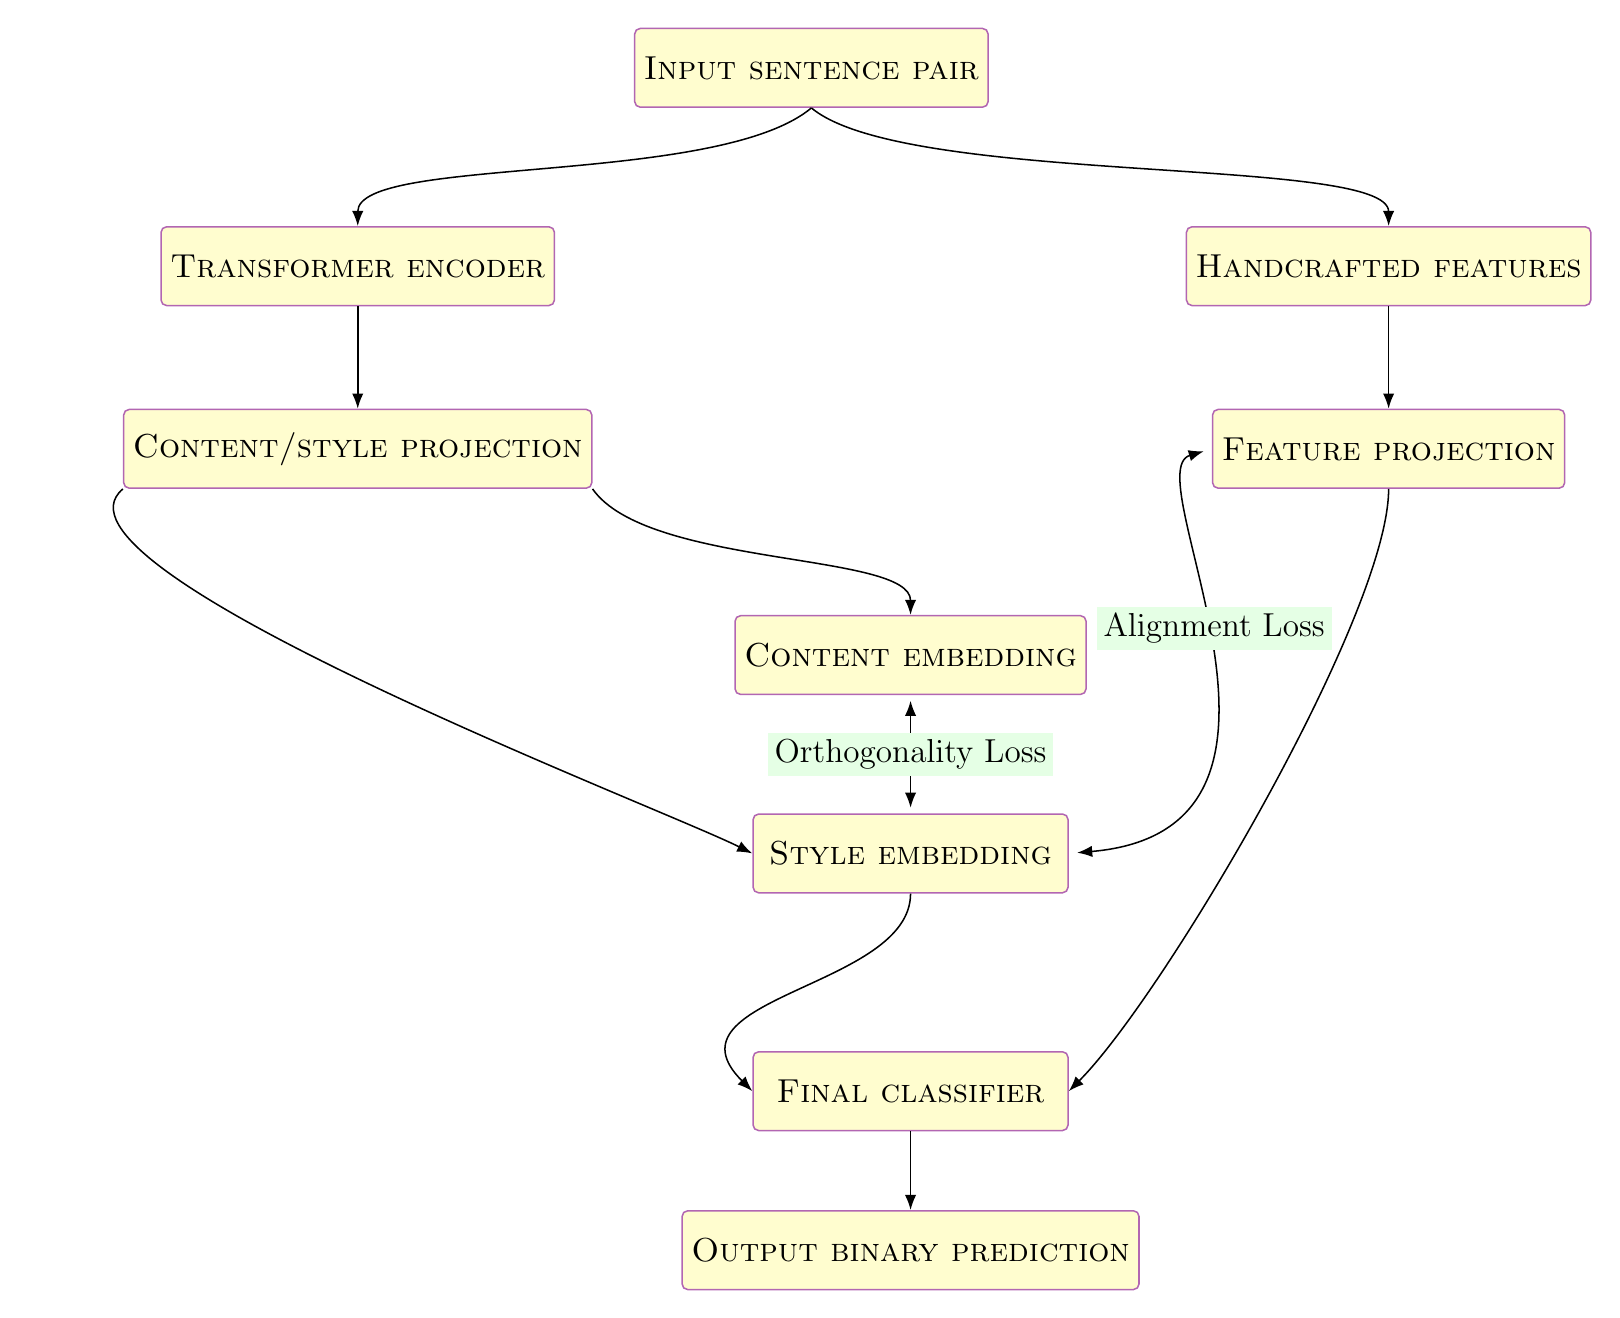
\begin{tikzpicture}[
  >=Latex,                          
  font=\large,
  line width=0.55pt,
  bend angle=18,
  box/.style={
     draw=violet!60,
     %use violet!10 for the first version, change for poster!
     fill=yellow!19,
     rounded corners=2pt,
     minimum width=4cm,
     minimum height=1cm,
     align=center
  },
  loss/.style={
     fill=green!10,
     inner sep=2.5pt,
     align=center
  }
]

\node[box] (input)                      {\textsc{Input sentence pair}};

\node[box, below left = 1.5cm and 1cm of input] (trans) {\textsc{Transformer encoder}};
\node[box, below            = 1.3cm of trans]             (proj)  {\textsc{Content/style projection}};

\node[box, below right= 1.6cm and 1.8cm of proj] (cont)   {\textsc{Content embedding}};
\node[box, below            = 1.5cm of cont]              (style) {\textsc{Style embedding}};

\node[box, below right= 1.5cm and 2.5cm of input] (hand)  {\textsc{Handcrafted features}};
\node[box, below            = 1.3cm of hand]              (feat)  {\textsc{Feature projection}};

\node[box, below            = 2.0cm of style]             (final) {\textsc{Final classifier}};
\node[box, below            = 1cm of final]             (out)   {\textsc{Output binary prediction}};


\draw[->] (input.south)  .. controls +(-1.2,-1.0) and +(0, 0.9) ..  (trans.north);
\draw[->] (input.south)  .. controls +( 1.2,-1.0) and +(0, 0.9) ..  (hand.north);


\draw[->] (trans) -- (proj);
\draw[->] (proj.south east) .. controls +( 0.7,-1.0) and +(0, 0.8) .. (cont.north);

\draw[<->, shorten >=2pt, shorten <=2pt]          
     (cont) -- (style)
     node[midway, loss] {Orthogonality Loss};


\draw[->] (proj.south west)  .. controls +(-1.2,-1.0) and +(-1.2, 0.6) .. (style.west);


\draw[->] (style.south)      .. controls +( 0,-1.2) and +(-1.2, 1.2) .. (final.west);


\draw[->] (hand) -- (feat);


\draw[<->, shorten >=3pt, shorten <=3pt]   
      (style.east) 
      .. controls +(3.5,0.3) and +(-1,-0.3) ..
      (feat.west)
      node[midway, loss, above] {Alignment Loss};


\draw[->] (feat.south)       .. controls +( 0,-1.6) and +( 1.2, 1.2) .. (final.east);


\draw[->] (final) -- (out);

\end{tikzpicture}
\end{document}